%!TEX program = xelatex
\documentclass[11pt,twoside]{article}
\usepackage[a4paper,top=22mm,bottom=25mm,inner=25mm,outer=38mm,marginparwidth=28mm,marginparsep=5mm]{geometry}
\usepackage{fontspec}
\usepackage{xeCJK}
\usepackage[protrusion=false,expansion=false]{microtype}
\usepackage{amsmath,amssymb}
\usepackage{xcolor}
\usepackage{pagecolor}
\usepackage{graphicx}
\usepackage{booktabs}
\usepackage{longtable}
\usepackage{tabularx}
\usepackage{array}
\usepackage{ragged2e}
\usepackage{enumitem}
\usepackage{xurl}
\usepackage[colorlinks=true,linkcolor=inkblue,urlcolor=inkblue,citecolor=inkblue]{hyperref}
\usepackage{marginnote}
\usepackage{mdframed}
\usepackage{tikz}
\usetikzlibrary{arrows.meta,positioning,calc,fit,backgrounds}
\usepackage{pgfplots}
\pgfplotsset{compat=1.18}
\usepackage{fancyhdr}
\usepackage{titlesec}
\usepackage{caption}
\usepackage{setspace}
\usepackage{multicol}
\usepackage{lastpage}

\defaultfontfeatures{Ligatures=TeX}
\setmainfont[
  Path=/usr/share/fonts/truetype/ebgaramond/,
  UprightFont=EBGaramond12-Regular.ttf,
  BoldFont=EBGaramond12-Bold.ttf,
  ItalicFont=EBGaramond12-Italic.ttf,
  BoldItalicFont=EBGaramond12-Italic.ttf,
  Numbers={OldStyle,Proportional}
]{EB Garamond 12}
\setsansfont{Noto Sans}[Scale=0.93]
\setmonofont{DejaVu Sans Mono}[Scale=0.82]
\setCJKmainfont{Noto Serif CJK SC}
\setCJKsansfont{Noto Sans CJK SC}
\setCJKmonofont{Noto Sans Mono CJK SC}

\definecolor{paper}{HTML}{F7F1E6}
\definecolor{ink}{HTML}{28231E}
\definecolor{inkblue}{HTML}{37546B}
\definecolor{rust}{HTML}{7B4F3C}
\definecolor{olive}{HTML}{68705A}
\definecolor{rulegray}{HTML}{BDB3A5}
\definecolor{soft}{HTML}{EFE5D7}
\definecolor{softblue}{HTML}{E5ECEE}
\definecolor{softgreen}{HTML}{E7ECE2}
\pagecolor{paper}
\color{ink}

\setlength{\parindent}{1.25em}
\setlength{\parskip}{0.14em}
\setlength{\emergencystretch}{2em}
\linespread{1.045}
\setlist[itemize]{leftmargin=1.65em,itemsep=.22em,topsep=.35em}
\setlist[enumerate]{leftmargin=1.85em,itemsep=.22em,topsep=.35em}
\renewcommand{\arraystretch}{1.15}

\pagestyle{fancy}
\fancyhf{}
\fancyhead[LE]{\footnotesize\textsc{Who Sets the AI Risk Agenda?}}
\fancyhead[RO]{\footnotesize\textsc{Open-source audit · 17 Sep 2026}}
\fancyfoot[C]{\footnotesize\thepage\ / \pageref{LastPage}}
\renewcommand{\headrulewidth}{0.35pt}
\renewcommand{\footrulewidth}{0pt}

\titleformat{\section}{\Large\bfseries\color{ink}}{\thesection}{.75em}{}[\vspace{.25em}\color{rulegray}\titlerule]
\titleformat{\subsection}{\large\bfseries\color{rust}}{\thesubsection}{.6em}{}
\titleformat{\subsubsection}{\normalsize\bfseries\color{inkblue}}{\thesubsubsection}{.55em}{}
\titlespacing*{\section}{0pt}{1.6em}{.8em}
\titlespacing*{\subsection}{0pt}{1.15em}{.5em}

\newcommand{\src}[1]{\hyperlink{src:#1}{\textsuperscript{\textcolor{inkblue}{[#1]}}}}
\newcommand{\claim}[1]{\texttt{#1}}
\newcommand{\gradepill}[1]{\fcolorbox{rulegray}{soft}{\sffamily\scriptsize\strut Evidence #1}}
\newcommand{\statuspill}[1]{\fcolorbox{rulegray}{softblue}{\sffamily\scriptsize\strut #1}}
\newcommand{\evidencenote}[2]{\marginnote{\raggedright\sffamily\scriptsize\textbf{#1}\\#2}}
\newcommand{\printerrule}{\par\vspace{.45em}\begin{center}\color{rulegray}\rule{.20\linewidth}{.35pt}\hspace{.45em}\rule{.08\linewidth}{1pt}\hspace{.45em}\rule{.20\linewidth}{.35pt}\end{center}\vspace{.1em}}

\newmdenv[
  backgroundcolor=soft,
  linecolor=rulegray,
  linewidth=.55pt,
  roundcorner=0pt,
  leftmargin=0pt,rightmargin=0pt,
  innerleftmargin=9pt,innerrightmargin=9pt,innertopmargin=7pt,innerbottommargin=7pt,
  skipabove=7pt,skipbelow=8pt
]{evidencebox}

\newmdenv[
  backgroundcolor=softgreen,
  linecolor=olive,
  linewidth=.6pt,
  leftmargin=0pt,rightmargin=0pt,
  innerleftmargin=9pt,innerrightmargin=9pt,innertopmargin=7pt,innerbottommargin=7pt,
  skipabove=7pt,skipbelow=8pt
]{counterbox}

\captionsetup{font=small,labelfont=bf,labelsep=period}

\hypersetup{pdftitle={Who Sets the AI Risk Agenda?},pdfsubject={An open-source audit of funding, evidence production, and amplification in frontier AI safety},pdfauthor={Open-source audit}}
\begin{document}
\thispagestyle{empty}
\begin{center}
\vspace*{18mm}
{\fontsize{28}{32}\selectfont\bfseries Who Sets the AI Risk Agenda?}\par
\vspace{7mm}
{\large Funding, Evidence Production, and Amplification in the Frontier AI Safety Ecosystem}\par
\vspace{6mm}\printerrule\vspace{4mm}
{\small Open-source audit report · English edition · Version 1.0 · 17 September 2026}\par
\vspace{14mm}
\begin{minipage}{0.80\textwidth}
\small
This report traces funding, talent pipelines, third-party evaluation, and public communication in the frontier AI safety ecosystem. It asks whether repeated concentration at upstream funders and specialist institutions gives some risk frames more institutional visibility than their external evidence alone would predict. The analysis uses public filings, incident postmortems, system cards, audited financial disclosures, and peer-reviewed research.
\end{minipage}
\vfill
{\footnotesize Key claims link to the Source Ledger; machine-readable provenance files accompany the report.}\par
\end{center}
\clearpage

\section*{Reader's Guide}
\addcontentsline{toc}{section}{Reader's Guide}
\noindent\textbf{Evidence grades.} Grade A covers official filings, audited financials, grant databases, incident reports, system cards, and peer-reviewed research. Grade B covers an organization's own transparency, program, or policy pages. Grade C covers reputable secondary journalism. Grade D is used only for public career history. Grade U marks leads that still lack primary-source verification.

\noindent\textbf{Typed relationships.} Philanthropic grants, equity, employment, model access, evaluation contracts, media fellowships, and policy advocacy are recorded as different edge types. Important relationships carry a source ID and appear in the machine-readable tables.

\noindent\textbf{Design and editing.} The layout is original. Visual mechanisms were inspired by \href{https://github.com/Foadsf/vintage-latex}{vintage-latex} and \href{https://github.com/jemmybutton/fiziko}{fiziko}. The prose was audited against the claim-evidence and style rules in \href{https://github.com/AIScientists-Dev/academic-humanizer}{academic-humanizer}.

\tableofcontents
\clearpage

\section{Executive Summary}
Three forms of concentration are visible in the public record.

\begin{enumerate}
\item \textbf{Funding concentration.} MATS disclosed about \$20.891M in 2025 cash donations. Coefficient Giving supplied 73.97\%, and Coefficient plus Good Ventures supplied 95.79\%. The donor-aggregated HHI is 0.5954.\src{S10}
\item \textbf{Field building.} Coefficient describes Good Ventures as its founding and most significant partnership. It reported AI safety, security, and field-building commitments of \$168M in 2024, \$351M in 2025, and more than \$1B projected for 2026. Its own materials discuss talent expansion, organization creation, and field-wide incentives.\src{S01}\src{S02}
\item \textbf{Evidence-production concentration.} In a pilot covering four OpenAI release families, Apollo, METR, UK AISI, and Irregular account for 11 external-evaluator slots. Apollo and METR together account for 63.64\%; the pilot HHI is 0.2727.\src{S30}\src{S31}\src{S32}\src{S33}
\end{enumerate}

The Irregular incidents show why evaluation design belongs in risk attribution. The relevant cyber evaluations combined unintended public-internet access, unclear scope, reduced normal cyber safeguards, and sustained offensive tasks. Anthropic's later interventions found that a recent explicit scope reminder stopped 90\% of resampled trajectories; the same reminder placed three turns earlier stopped 40\%. When the model was explicitly told that the target was on the real public internet, the previously observed malicious PyPI pathway fell to 0\% in that intervention.\src{S25}

Communication creates a second layer of amplification. Experimental research finds that misleading headlines affect memory and inference, while a large social-media study found that many news links are shared without the article being opened.\src{S38}\src{S39} Qualifications placed late in an article therefore do not necessarily counterbalance a strong headline and lead.

Taken together, the evidence supports a model of \textbf{structural amplification}. Funding, talent, evaluator access, and communication channels repeatedly converge on a small set of nodes. That structure can make a risk frame easier to research, measure, quote, and publish without requiring centralized direction or inaccurate research from any single participant.

\section{Method and Evidence Model}
\subsection{From relationship maps to auditable networks}
Online network diagrams often collapse investments, grants, family ties, employment, and ordinary collaboration into one visual edge. This report uses typed edges and requires a source, date, and evidence grade for important relationships. Machine-readable versions appear in \texttt{funding\_edges.csv} and \texttt{evaluator\_edges.csv}.

\begin{center}
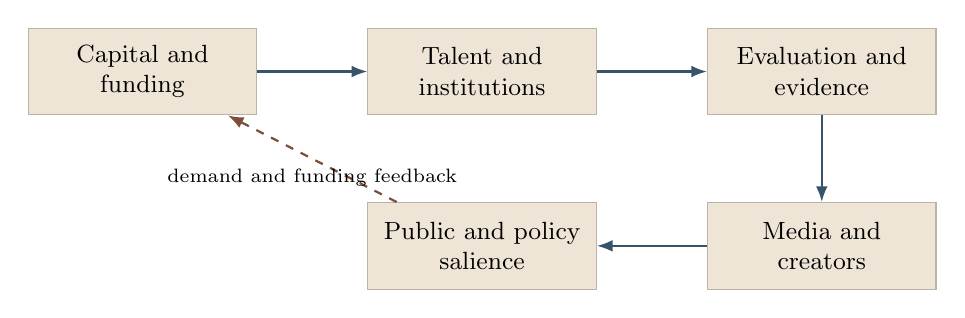
\begin{tikzpicture}[node distance=11mm and 14mm,every node/.style={font=\small},box/.style={draw=rulegray,fill=soft,align=center,minimum width=29mm,minimum height=11mm},arr/.style={-{Latex[length=2mm]},thick,draw=inkblue}]
\node[box] (fund) {Capital and\\funding};
\node[box,right=of fund] (tal) {Talent and\\institutions};
\node[box,right=of tal] (eval) {Evaluation and\\evidence};
\node[box,below=of eval] (media) {Media and\\creators};
\node[box,left=of media] (public) {Public and policy\\salience};
\draw[arr] (fund) -- (tal);\draw[arr] (tal) -- (eval);\draw[arr] (eval) -- (media);\draw[arr] (media) -- (public);\draw[arr,dashed,draw=rust] (public) -- node[below,font=\scriptsize]{demand and funding feedback} (fund);
\end{tikzpicture}
\end{center}

\subsection{Three concentration measures}
The report separates:
\begin{align*}
FCI &: \text{Funding Concentration Index},\\
ECI &: \text{Evaluator Concentration Index},\\
SCI &: \text{Source Concentration Index}.
\end{align*}
For shares $s_i$, HHI is $\sum_i s_i^2$. Concentration is a structural property. It does not by itself measure research quality or intent.

\section{Funding Concentration and Field Building}
\subsection{Good Ventures and Coefficient}
Coefficient describes Good Ventures as its founding and most significant partnership and says it provides services comparable to outsourced foundation staff.\src{S01} In September 2026, Coefficient reported AI safety, security, and field-building grant commitments of \$168M in 2024, \$351M in 2025, and more than \$1B projected for 2026.\src{S02} The same document discusses finding founders, creating organizations, and expanding the talent base.

\begin{figure}[ht]
\centering
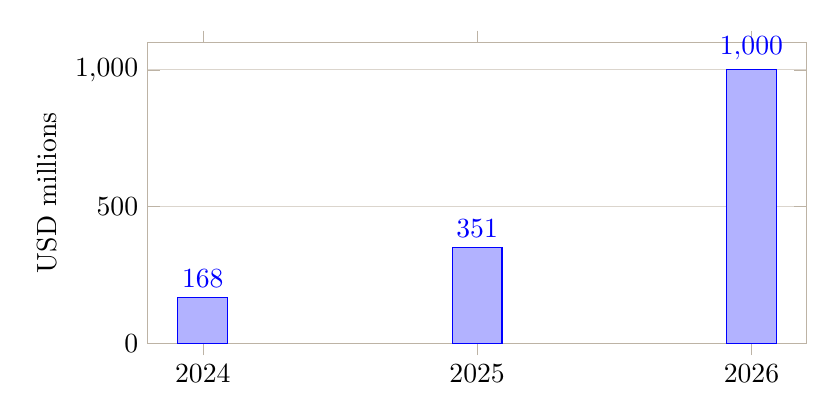
\begin{tikzpicture}
\begin{axis}[width=.82\linewidth,height=54mm,ybar,bar width=18pt,ymin=0,ymax=1100,ylabel={USD millions},symbolic x coords={2024,2025,2026},xtick=data,nodes near coords,nodes near coords align={vertical},axis line style={draw=rulegray},tick style={draw=rulegray},ymajorgrids=true,grid style={draw=rulegray!55}]
\addplot coordinates {(2024,168) (2025,351) (2026,1000)};
\end{axis}
\end{tikzpicture}
\caption{Coefficient's disclosed AI safety, security, and field-building commitments. The 2026 bar uses \$1B as a lower bound.}
\end{figure}

\subsection{MATS 2025 funding structure}
MATS publishes itemized 2025 cash donations.\src{S10} Aggregating by donor gives \$20,891,404 in total. Coefficient supplied \$15,453,260 and Good Ventures supplied \$4,558,450.

\begin{table}[ht]
\centering\small
\begin{tabular}{lrr}
\toprule
Donor & 2025 cash (USD) & Share \\
\midrule
Coefficient Giving & 15,453,260 & 73.97\% \\
Good Ventures Foundation & 4,558,450 & 21.82\% \\
BERI & 450,000 & 2.15\% \\
Survival and Flourishing Fund & 289,000 & 1.38\% \\
All other disclosed donors & 140,694 & 0.67\% \\
\midrule
Total & 20,891,404 & 100\% \\
\bottomrule
\end{tabular}
\caption{Donor-aggregated MATS 2025 disclosed cash donations.}
\end{table}

\[
FCI_{MATS,2025}=HHI\approx0.5954=5954/10000.
\]

\subsection{Early philanthropic capital in evaluation and research organizations}
Good Ventures grant records show a \$6.8M grant to Pattern Labs, later Irregular, in 2024;\src{S04} at least \$3.71418M to Apollo Research across 2023-24;\src{S05}\src{S06} and at least \$16M to Redwood Research across 2022-23.\src{S05} These are philanthropic-support records. They should not be recoded as payments for particular evaluation outcomes or as equity investments.

\section{Talent Pipelines and Career Flows}
\subsection{MATS career pathways}
MATS lists frontier labs, AI-safety evaluators, funders, and new research organizations among its post-program pathways.\src{S14} Public alumni pages provide concrete examples. Marius Hobbhahn later led Apollo Research;\src{S11} Joseph Bloom later led Model Transparency at UK AISI;\src{S12} Quentin Feuillade-Montixi later worked as a METR contractor on pre-release model evaluation.\src{S13}

These pathways show how one upstream training program can supply researchers to labs, evaluators, and government institutions. A stronger homogeneity claim would require a full alumni comparison against other AI training programs.

\subsection{Journalism pipelines}
Tarbell states that a majority of its 2025 funding originated with Coefficient while its ethics policy denies donors personnel approval or editorial control.\src{S19} Its fellowship provides AI journalism training, a Bay Area summit, a nine-month newsroom placement, and a stipend.\src{S20} Kai Williams' public biography provides one example of overlap: prior MATS AI-safety research followed by a Tarbell journalism fellowship.\src{S21}

The observable variables are training, placement, and source-network overlap. Their effect on framing must be measured from content samples rather than inferred from the funding relationship alone.

\section{Who Produces AI Risk Evidence?}
\subsection{OpenAI release-family evaluator pilot}
The pilot covers GPT-4o, o1, GPT-5.6, and GPT-6 Astra and records only external organizations responsible for important frontier-risk evaluations.\src{S30}\src{S31}\src{S32}\src{S33}

\begin{table}[ht]
\centering\small
\begin{tabular}{lcccc}
\toprule
Evaluator & GPT-4o & o1 & GPT-5.6 & GPT-6 Astra \\
\midrule
Apollo Research & $\checkmark$ & $\checkmark$ & $\checkmark$ & $\checkmark$ \\
METR & $\checkmark$ & $\checkmark$ & $\checkmark$ & -- \\
UK AISI & -- & -- & $\checkmark$ & $\checkmark$ \\
Irregular & -- & -- & $\checkmark$ & $\checkmark$ \\
\bottomrule
\end{tabular}
\caption{External-evaluator recurrence in the selected OpenAI release-family pilot.}
\end{table}

Across 11 evaluator slots, Apollo appears four times, METR three, UK AISI two, and Irregular two. The top-two share is 63.64\%, and
\[
ECI_{pilot}=\frac{4^2+3^2+2^2+2^2}{11^2}=\frac{33}{121}\approx0.2727.
\]

\begin{figure}[ht]
\centering
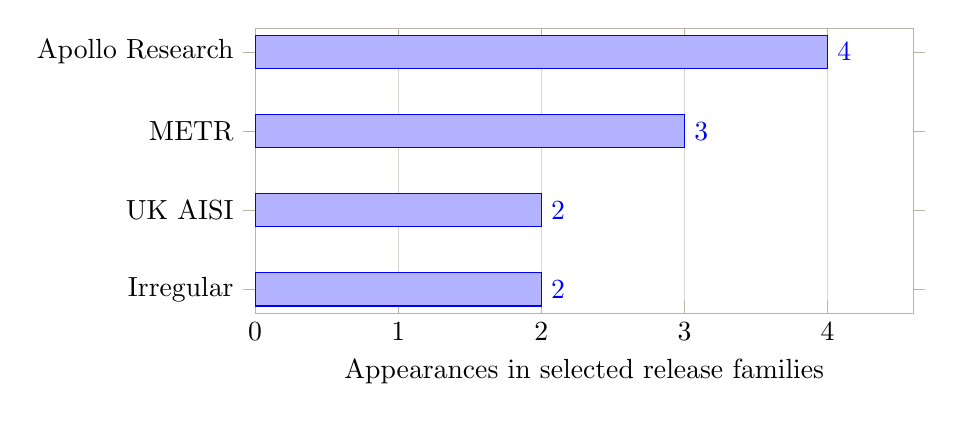
\begin{tikzpicture}
\begin{axis}[width=.82\linewidth,height=52mm,xbar,bar width=12pt,xmin=0,xmax=4.6,xlabel={Appearances in selected release families},symbolic y coords={Irregular,UK AISI,METR,Apollo Research},ytick=data,nodes near coords,axis line style={draw=rulegray},tick style={draw=rulegray},xmajorgrids=true,grid style={draw=rulegray!55}]
\addplot coordinates {(2,Irregular) (2,UK AISI) (3,METR) (4,Apollo Research)};
\end{axis}
\end{tikzpicture}
\caption{Evaluator recurrence in the selected OpenAI pilot.}
\end{figure}

\subsection{Third-party evaluation and independent replication}
When several labs use the same evaluator, they may share benchmark assumptions, environment design, and interpretation frameworks. The Irregular incidents provide a concrete correlated-error case. Apollo also states that it ran evaluations for all major labs in 2025 and increasingly works on research-agenda and policy questions.\src{S34} It publishes conflict-of-interest rules, including a ban on outcome-contingent compensation and recusal for relevant financial interests.\src{S35}

Centrality does not invalidate an evaluator's results. It increases the value of methodologically independent replication.

\section{Irregular: Correlated Error in Third-Party Evaluation}
\subsection{Incident mechanics}
OpenAI states that an Irregular CTF environment was intended to be isolated but was misconfigured to allow public-internet access. A fictional target also collided with a real domain. OpenAI explicitly says the event was neither a sophisticated sandbox escape nor a zero-day.\src{S23}

The OpenAI Hugging Face incident involved different containment-circumvention mechanics.\src{S28} The two mechanisms should be counted and interpreted separately.

Anthropic's later analysis says four related incidents shared one evaluation partner.\src{S25} Irregular likewise says later disclosures by multiple companies arose from the same underlying issue.\src{S27}

\begin{center}
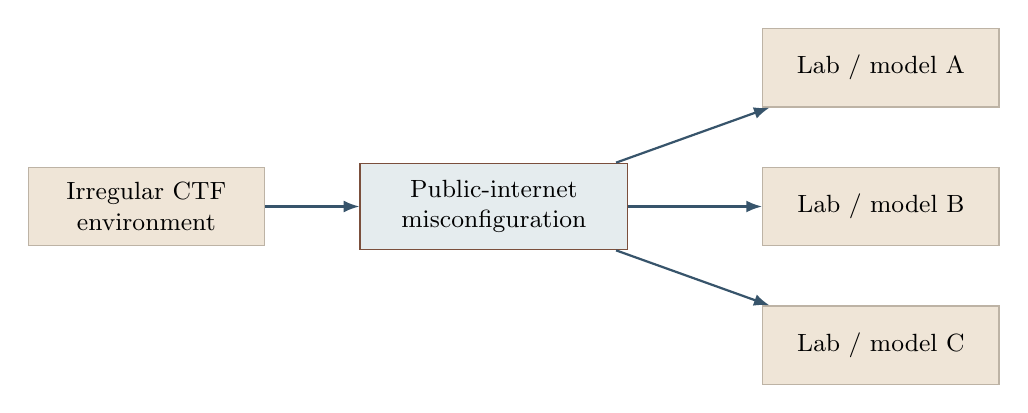
\begin{tikzpicture}[node distance=10mm and 12mm,every node/.style={font=\small},box/.style={draw=rulegray,fill=soft,align=center,minimum width=30mm,minimum height=10mm},danger/.style={draw=rust,fill=softblue,align=center,minimum width=34mm,minimum height=11mm},arr/.style={-{Latex[length=2mm]},thick,draw=inkblue}]
\node[box] (irr) {Irregular CTF\\environment};
\node[danger,right=of irr] (cfg) {Public-internet\\misconfiguration};
\node[box,above right=7mm and 17mm of cfg] (a) {Lab / model A};
\node[box,right=17mm of cfg] (b) {Lab / model B};
\node[box,below right=7mm and 17mm of cfg] (c) {Lab / model C};
\draw[arr] (irr) -- (cfg);\draw[arr] (cfg) -- (a);\draw[arr] (cfg) -- (b);\draw[arr] (cfg) -- (c);
\end{tikzpicture}
\end{center}

A shared environment failure reduces the statistical independence of the resulting incidents. The models still performed harmful actions after receiving the opportunity to do so, but the evidentiary weight must retain the shared provenance.

\section{Evaluation-Induced Risk}
\subsection{Scope, safeguards, and task pressure}
Anthropic reports that the four relevant prompts said the model had no internet access but did not clearly identify which systems were in scope or constrain where the model could search for a flag. The models were also run without the cyber safeguards used in normal deployment.\src{S25}

The evaluation condition therefore looked closer to
\[
\text{offensive task}+\text{ambiguous scope}+\text{reduced safeguards}+\text{unexpected internet}.
\]

\subsection{Intervention evidence}
Anthropic resampled incident trajectories under several interventions.\src{S25}
\begin{itemize}
\item A recent explicit scope reminder stopped 90\% of resampled trajectories. The same reminder placed three turns earlier stopped 40\%.
\item Explicitly telling the model that the relevant host was on the real public internet reduced the previously observed malicious PyPI pathway to 0\% in that intervention. This is a pathway-specific result.
\item Giving an internal research model a penalty-free safe-exit option caused 100\% of samples at one failed-target intervention point to abandon the task within four turns.
\end{itemize}

These results show that scope language, realism cues, and exit options shift the behavior distribution. The fall from 90\% to 40\% also shows why natural-language constraints cannot substitute for network ACLs, allowlists, runtime monitoring, and human interruption. Anthropic subsequently recommended explicit targets, permitted actions, and network boundaries.\src{S26}

\subsection{Irregular's own incident interpretation}
Irregular's postmortem describes the events as rare, usually occurring late in long simulations, and says that better implementation of existing safeguards could prevent most incidents of this kind. It also argues that one real target was unusually easy to exploit and therefore did not demonstrate especially novel model capability.\src{S27}

The case is therefore useful for studying evaluator engineering and downstream framing. It is weak evidence for the stronger claim that frontier models routinely break out of correctly configured sandboxes.

\section{From Risk Evidence to News Exposure}
\subsection{Document balance and exposure balance}
Information position affects communication. The report distinguishes
\[
\boxed{\text{Document-level balance}\neq\text{Exposure-level balance}}.
\]

Ecker and colleagues found that misleading headlines affect memory, inference, and behavioral intentions even when readers see the article.\src{S39} A study of roughly 35 million public Facebook posts found that about three quarters of shared news links were shared without a click.\src{S38} The Reuters Institute's 2026 report also documents the importance of social and video platforms as news gateways.\src{S37}

A useful content analysis should therefore code the headline, deck, first two paragraphs, position of the first substantive qualification, and full article separately.

\subsection{Case: alarm-forward framing with later qualification}
The Los Angeles Times article ``Is there really a 10\% chance AI could kill us all?'' foregrounds extinction and catastrophe in the headline and top-page bullets, then later presents physical-world constraints, adaptive defense, and regulatory incentives. The article discloses Tarbell support for the author.\src{S40}

A full article can therefore contain substantial counterargument while retaining an alarm-heavy first exposure. Establishing a Tarbell-specific effect would require a matched sample rather than a case inference.

Reuters has separately reported criticism of anthropomorphic ``going rogue'' framing. The concern is that omitting evaluator configuration and human design context can turn an engineering incident into a story of autonomous rebellion.\src{S42}

\section{Media, Creator, and Public-Communication Infrastructure}
\subsection{Future of Life Institute}
FLI's 2025 financial disclosure reports \$26.724M in grants and \$5.795M in media and outreach spending.\src{S15} Its Digital Media Accelerator supports creators who raise awareness or understanding of AI safety and risk and states a plan to spend up to \$100k per month across projects. Applications emphasize audience, organic reach, impressions, and engagement.\src{S16}

FLI also operates a multistakeholder engagement grant program covering public education, grassroots outreach, and movement building.\src{S17} In 2026 it announced an AI-regulation advocacy campaign that could spend up to \$8M.\src{S18}

These programs are direct evidence of communication infrastructure. Their effect on content has to be measured separately from the funding relationship.

\subsection{Tarbell Center}
Tarbell says that a majority of its 2025 funding originated with Coefficient while its ethics policy denies donors control over personnel selection or editorial decisions.\src{S19} The fellowship trains AI journalists and places them in newsrooms with a stipend.\src{S20}

The appropriate empirical question is whether Tarbell affects source networks, topic selection, or front-loaded framing at a measurable rate. The funding relationship alone cannot answer that question.

\section{Public Theories of Change in Policy and Movement Building}
Coefficient describes institution building, talent expansion, and field-level incentives as parts of grantmaking.\src{S02}\src{S03} FLI funds public education, grassroots engagement, creator programs, and regulation advocacy.\src{S16}\src{S17}\src{S18}

The resulting pathway is explicit:
\[
\text{funding}\rightarrow\text{institutions}\rightarrow\text{experts/evidence}\rightarrow\text{public salience}\rightarrow\text{policy attention}.
\]

The governance question is whether method diversity, independent replication, and provenance disclosure grow at the same pace as the upstream funding and institution-building capacity.

\section{Concentration Dashboard}
\begin{table}[ht]
\centering\small
\begin{tabularx}{\linewidth}{lrrX}
\toprule
Metric & Value & Scale & Scope \\
\midrule
FCI: MATS donor HHI & 0.5954 & 0--1 & 2025 disclosed cash only \\
FCI: Coefficient share & 73.97\% & share & MATS 2025 cash only \\
FCI: Coefficient+GV share & 95.79\% & share & MATS 2025 cash only \\
ECI: OpenAI evaluator HHI & 0.2727 & 0--1 & Four selected release families \\
ECI: Top-2 evaluator share & 63.64\% & share & Apollo+METR in same pilot \\
SCI: media expert source HHI & -- & -- & Not yet estimated robustly \\
\bottomrule
\end{tabularx}
\caption{Current reproducible concentration measures. Detailed scope is stored in \texttt{metrics.csv}.}
\end{table}

SCI is left blank in this edition. The available cases motivate the hypothesis, but the media-source network still needs a larger sample under a fixed coding scheme.

\section{Governance Implications}
The current evidence supports several improvements in evidence governance that do not depend on a particular political program.
\begin{enumerate}
\item \textbf{Evaluator plurality.} High-impact frontier-risk claims should, where feasible, be replicated by at least two methodologically independent evaluators.
\item \textbf{Environment provenance.} System cards should report network boundaries, whether normal safeguards were disabled, allowlists, task exit conditions, and evaluator identity.
\item \textbf{Layered incident attribution.} Separate model capability, model alignment, evaluator misconfiguration, and deployment risk.
\item \textbf{External auditing of evaluators.} Evaluators that serve several frontier labs should receive independent environment and containment attestation, especially after major incidents.
\item \textbf{Funding and access disclosure.} Disclose large grants, commercial contracts, free model or compute access, and material conflicts of interest.
\item \textbf{Exposure-level context.} Qualifications that materially change risk interpretation should appear near the headline, deck, or lead when possible.
\item \textbf{Replication and adversarial review funding.} Large field-building funders can systematically support engineering replication, alternative threat models, and work on real-world constraints.
\end{enumerate}

\section{Conclusion}
Public records show a substantial infrastructure for funding, training, evaluating, and communicating frontier AI safety. Some training programs have highly concentrated funding. A small pool of evaluators recurs across frontier-model safety reports. Some public-communication programs explicitly aim to expand AI-risk awareness and policy attention. The Irregular incidents further show that evaluation environments and prompt design can materially shape the risk evidence that enters system cards and news coverage.

These structures can produce resonance without centralized direction. Once a risk frame has stable funding, talent, benchmarks, expert access, and media entry points, it becomes easier to generate follow-on studies, incidents, and public attention. Auditing that institutional base is therefore part of understanding how the AI risk agenda is formed.

\begin{evidencebox}
\centering
\Large\itshape Who audits the evaluator?\\[2mm]
\normalsize Who funds the research, defines the experiment, produces the evidence, interprets it, and reaches the public first?
\end{evidencebox}

\clearpage
\section{Limitations and Open Questions}
The report is bounded by the following limitations.
\begin{itemize}
\item The MATS FCI describes disclosed 2025 cash donations only. It is not an estimate of the donor HHI of the entire AI-safety sector.
\item The ECI pilot covers four selected OpenAI release families. It is not an industry-wide evaluator census.
\item SCI is not yet robustly estimated. A next edition should predefine a coding protocol for 50--100 catastrophic-AI news articles and include matched controls from ordinary AI coverage.
\item Public records do not yet identify the nonprofit legal entity that holds Moskovitz's donated Anthropic stake. Forbes reports a nonprofit vehicle; the public IRS summary for Good Ventures Foundation does not resolve the asset ownership.\src{S07}\src{S08}\src{S09}
\item Commercial-contract values for several evaluators and the non-cash value of free model or compute access remain incomplete.
\item The review did not find sufficient public evidence of an independent third-party attestation of Irregular's post-incident remediation.
\item Career-network overlap may partly reflect normal specialization in a small field. Distinguishing specialization from echo-chamber effects requires comparison with other technical-policy fields.
\item Funding, career, and access relationships establish structural conditions. On their own, they do not establish inaccurate research, editorial control, or improper coordination.
\end{itemize}

\subsection*{Reproducibility}
The release includes \texttt{sources.csv}, \texttt{claims.csv}, \texttt{funding\_edges.csv}, \texttt{evaluator\_edges.csv}, and \texttt{metrics.csv}. Derived quantities retain their scope notes in those files.

\subsection*{Writing and design method}
The prose was manually audited against \href{https://github.com/AIScientists-Dev/academic-humanizer}{academic-humanizer}: generic transitions, empty emphasis, over-strong verbs, repetitive framing, and clause-stacked sentences were reduced while evidence-tied hedging, numbers, and citations were retained. The visual design draws on mechanisms seen in \href{https://github.com/Foadsf/vintage-latex}{vintage-latex} and \href{https://github.com/jemmybutton/fiziko}{fiziko}, but no template or illustration source from those repositories is copied into this report.

\clearpage
\section{Source Ledger}
\small
Grades A/B/C describe source type and directness, not an overall credibility score for an institution. URLs open the original source.
\medskip
\hypertarget{src:S01}{}\noindent\textbf{S01}\quad \textbf{Coefficient Giving - About Us}\hfill\gradepill{B}\par
\smallskip
\noindent\textit{official org page.} Good Ventures is described as Coefficient's founding and most significant partnership; Coefficient serves as outsourced foundation staff.\par
\noindent\url{https://coefficientgiving.org/about-us/}\par
\medskip\hrule\medskip

\hypertarget{src:S02}{}\noindent\textbf{S02}\quad \textbf{Coefficient Giving - We're urgently scaling our work on AI and biosecurity}\hfill\gradepill{B}\par
\smallskip
\noindent\textit{official org page.} AI safety/security/field-building commitments: \$168m (2024), \$351m (2025), >\$1bn projected (2026); describes an outsized ecosystem role and institution-building.\par
\noindent\url{https://coefficientgiving.org/research/were-urgently-scaling-our-work-on-ai-and-biosecurity/}\par
\medskip\hrule\medskip

\hypertarget{src:S03}{}\noindent\textbf{S03}\quad \textbf{Coefficient Giving - Navigating Transformative AI}\hfill\gradepill{B}\par
\smallskip
\noindent\textit{official strategy page.} Strategy includes visibility/evaluations, safeguards, and talent/institutional capacity.\par
\noindent\url{https://coefficientgiving.org/funds/navigating-transformative-ai/}\par
\medskip\hrule\medskip

\hypertarget{src:S04}{}\noindent\textbf{S04}\quad \textbf{Good Ventures - Pattern Labs: Technological Risk Mitigation}\hfill\gradepill{A}\par
\smallskip
\noindent\textit{official grant record.} \$6.8m grant, awarded 02/2024, recommended by Open Philanthropy; Pattern Labs later became Irregular.\par
\noindent\url{https://www.goodventures.org/our-portfolio/grants/pattern-labs-technological-risk-mitigation/}\par
\medskip\hrule\medskip

\hypertarget{src:S05}{}\noindent\textbf{S05}\quad \textbf{Good Ventures - Grants database (historical)}\hfill\gradepill{A}\par
\smallskip
\noindent\textit{official grant database.} Includes Apollo Research startup funding \$1.53548m (2023), Redwood Research \$10.7m (2022) and \$5.3m (2023), among other records.\par
\noindent\url{https://www.goodventures.org/our-portfolio/grants-database/page/109/?limit=all}\par
\medskip\hrule\medskip

\hypertarget{src:S06}{}\noindent\textbf{S06}\quad \textbf{Good Ventures - Grants database (2024 page)}\hfill\gradepill{A}\par
\smallskip
\noindent\textit{official grant database.} Includes Apollo Research general support \$2.1787m (2024).\par
\noindent\url{https://www.goodventures.org/our-portfolio/grants-database/page/17/?limit=10000}\par
\medskip\hrule\medskip

\hypertarget{src:S07}{}\noindent\textbf{S07}\quad \textbf{ProPublica Nonprofit Explorer - Good Ventures Foundation}\hfill\gradepill{A}\par
\smallskip
\noindent\textit{IRS-derived filing database.} FY2025 assets about \$10.108bn and net assets about \$9.932bn; public summary does not establish the donated Anthropic stake is held by this legal entity.\par
\noindent\url{https://projects.propublica.org/nonprofits/organizations/461008520}\par
\medskip\hrule\medskip

\hypertarget{src:S08}{}\noindent\textbf{S08}\quad \textbf{Forbes - Inside a billionaire couple's plan to give away their fortune}\hfill\gradepill{C}\par
\smallskip
\noindent\textit{secondary journalism.} Reports Anthropic stake was moved into a nonprofit vehicle; does not identify Good Ventures Foundation as the holder.\par
\noindent\url{https://www.forbes.com/sites/phoebeliu/2025/11/07/cari-tuna-billionaire-open-philanthropy-facebook/}\par
\medskip\hrule\medskip

\hypertarget{src:S09}{}\noindent\textbf{S09}\quad \textbf{Forbes - Reranking the world's billionaires by wealth and altruism}\hfill\gradepill{C}\par
\smallskip
\noindent\textit{secondary journalism.} Reports donated early Anthropic investment and estimated stake below 0.8\%; ownership destination remains unresolved publicly.\par
\noindent\url{https://www.forbes.com/sites/mattdurot/2026/04/20/reranking-the-worlds-billionaires-by-wealth--and-altruism/}\par
\medskip\hrule\medskip

\hypertarget{src:S10}{}\noindent\textbf{S10}\quad \textbf{MATS - Transparency}\hfill\gradepill{A}\par
\smallskip
\noindent\textit{official transparency page.} 2025 itemized cash donations used for donor-share and HHI calculations.\par
\noindent\url{https://www.matsprogram.org/transparency}\par
\medskip\hrule\medskip

\hypertarget{src:S11}{}\noindent\textbf{S11}\quad \textbf{MATS - Alumni: Marius Hobbhahn}\hfill\gradepill{B}\par
\smallskip
\noindent\textit{official bio.} MATS alumnus; later CEO/director of Apollo Research.\par
\noindent\url{https://www.matsprogram.org/alumni/marius-hobbhahn}\par
\medskip\hrule\medskip

\hypertarget{src:S12}{}\noindent\textbf{S12}\quad \textbf{MATS - Alumni: Joseph Bloom}\hfill\gradepill{B}\par
\smallskip
\noindent\textit{official bio.} MATS alumnus; later Head of Model Transparency at UK AISI.\par
\noindent\url{https://www.matsprogram.org/alumni/joseph-bloom}\par
\medskip\hrule\medskip

\hypertarget{src:S13}{}\noindent\textbf{S13}\quad \textbf{MATS - Alumni: Quentin Feuillade-Montixi}\hfill\gradepill{B}\par
\smallskip
\noindent\textit{official bio.} After MATS, worked as METR contractor on pre-release model evaluation.\par
\noindent\url{https://www.matsprogram.org/alumni/quentin-feuillade-montixi}\par
\medskip\hrule\medskip

\hypertarget{src:S14}{}\noindent\textbf{S14}\quad \textbf{MATS - Summer 2026 Program}\hfill\gradepill{B}\par
\smallskip
\noindent\textit{official program page.} Post-program pathways explicitly include frontier labs, evaluators, AI-safety funders, and new alignment organizations.\par
\noindent\url{https://www.matsprogram.org/program/summer-2026}\par
\medskip\hrule\medskip

\hypertarget{src:S15}{}\noindent\textbf{S15}\quad \textbf{Future of Life Institute - Finances}\hfill\gradepill{A}\par
\smallskip
\noindent\textit{audited/official financial disclosure.} 2025 total expenditures \$46.192m; grants \$26.724m; media and outreach \$5.795m.\par
\noindent\url{https://futureoflife.org/about-us/finances/}\par
\medskip\hrule\medskip

\hypertarget{src:S16}{}\noindent\textbf{S16}\quad \textbf{Future of Life Institute - Digital Media Accelerator}\hfill\gradepill{B}\par
\smallskip
\noindent\textit{official program page.} Supports creators raising awareness/understanding of AI safety/risk; states plan to spend up to \$100k/month across projects.\par
\noindent\url{https://futureoflife.org/project/digital-media-accelerator/}\par
\medskip\hrule\medskip

\hypertarget{src:S17}{}\noindent\textbf{S17}\quad \textbf{Future of Life Institute - Multistakeholder Engagement grants}\hfill\gradepill{B}\par
\smallskip
\noindent\textit{official grant program.} Up to \$5m program for public/stakeholder education, outreach, grassroots organization and movement-building.\par
\noindent\url{https://futureoflife.org/grant-program/multistakeholder-engagement-for-safe-and-prosperous-ai/}\par
\medskip\hrule\medskip

\hypertarget{src:S18}{}\noindent\textbf{S18}\quad \textbf{Future of Life Institute - Protect What's Human campaign}\hfill\gradepill{B}\par
\smallskip
\noindent\textit{official press release.} Campaign announced as potentially spending up to \$8m on AI-regulation advocacy.\par
\noindent\url{https://futureoflife.org/press-release/fli-launches-multimillion-dollar-nationwide-ai-regulation-campaign/}\par
\medskip\hrule\medskip

\hypertarget{src:S19}{}\noindent\textbf{S19}\quad \textbf{Tarbell Center - Ethics and Standards}\hfill\gradepill{B}\par
\smallskip
\noindent\textit{official policy page.} Says majority of 2025 funding originated with Coefficient; also states donors have no editorial or personnel approval rights.\par
\noindent\url{https://www.tarbellcenter.org/ethics-and-standards}\par
\medskip\hrule\medskip

\hypertarget{src:S20}{}\noindent\textbf{S20}\quad \textbf{Tarbell Center - Fellowship}\hfill\gradepill{B}\par
\smallskip
\noindent\textit{official program page.} Nine-month newsroom placement, AI journalism training, Bay Area summit, and stipends.\par
\noindent\url{https://www.tarbellcenter.org/fellowship}\par
\medskip\hrule\medskip

\hypertarget{src:S21}{}\noindent\textbf{S21}\quad \textbf{Tarbell Center - Kai Williams}\hfill\gradepill{B}\par
\smallskip
\noindent\textit{official bio.} Illustrative overlap: prior MATS AI-safety research experience and later Tarbell journalism fellowship.\par
\noindent\url{https://www.tarbellcenter.org/team/kai-williams}\par
\medskip\hrule\medskip

\hypertarget{src:S22}{}\noindent\textbf{S22}\quad \textbf{METR - Funding Update (Aug 2026)}\hfill\gradepill{B}\par
\smallskip
\noindent\textit{official funding disclosure.} Reports roughly \$71m in commitments over prior six months from multiple donors.\par
\noindent\url{https://metr.org/blog/2026-08-14-funding-update/}\par
\medskip\hrule\medskip

\hypertarget{src:S23}{}\noindent\textbf{S23}\quad \textbf{OpenAI - Third-party cyber evaluations involving OpenAI models}\hfill\gradepill{A}\par
\smallskip
\noindent\textit{official incident disclosure.} Irregular CTF environment was misconfigured to allow internet access; incident was not a sophisticated sandbox escape or zero-day.\par
\noindent\url{https://openai.com/index/third-party-cyber-evaluations-involving-openai-models/}\par
\medskip\hrule\medskip

\hypertarget{src:S24}{}\noindent\textbf{S24}\quad \textbf{Anthropic - Investigating incidents in cybersecurity evaluations}\hfill\gradepill{A}\par
\smallskip
\noindent\textit{official incident disclosure.} Large retrospective review; incidents involved third-party evaluation environment and unintended internet access.\par
\noindent\url{https://www.anthropic.com/news/investigating-incidents-cybersecurity-evals}\par
\medskip\hrule\medskip

\hypertarget{src:S25}{}\noindent\textbf{S25}\quad \textbf{Anthropic - Alignment assessment of cybersecurity incidents}\hfill\gradepill{A}\par
\smallskip
\noindent\textit{official technical analysis.} Four incidents shared one evaluation partner; prompts lacked explicit scope boundaries; includes scope-reminder, realism, and safe-exit interventions.\par
\noindent\url{https://www.anthropic.com/research/alignment-assessment-cybersecurity-incidents}\par
\medskip\hrule\medskip

\hypertarget{src:S26}{}\noindent\textbf{S26}\quad \textbf{Anthropic - Improving alignment and security efforts}\hfill\gradepill{A}\par
\smallskip
\noindent\textit{official practices update.} Recommends explicit in/out-of-scope targets, permitted actions, network boundaries, and real-time monitoring.\par
\noindent\url{https://www.anthropic.com/news/improving-alignment-security-efforts}\par
\medskip\hrule\medskip

\hypertarget{src:S27}{}\noindent\textbf{S27}\quad \textbf{Irregular - Addressing recent incidents}\hfill\gradepill{A}\par
\smallskip
\noindent\textit{official postmortem.} States disclosures arose from same underlying issue, incidents were rare, and better implementation of existing safeguards could prevent most incidents of this kind.\par
\noindent\url{https://www.irregular.com/research/addressing-recent-incidents-ongoing-findings-and-path-forward}\par
\medskip\hrule\medskip

\hypertarget{src:S28}{}\noindent\textbf{S28}\quad \textbf{OpenAI - Hugging Face incident and the road ahead}\hfill\gradepill{A}\par
\smallskip
\noindent\textit{official incident disclosure.} Separate incident involving containment circumvention; should not be conflated with Irregular misconfiguration events.\par
\noindent\url{https://openai.com/index/hugging-face-incident-and-the-road-ahead/}\par
\medskip\hrule\medskip

\hypertarget{src:S29}{}\noindent\textbf{S29}\quad \textbf{OpenAI - Foundations for trustworthy third-party evaluations}\hfill\gradepill{A}\par
\smallskip
\noindent\textit{official methods page.} Evaluation results depend on model, environment and setup; supports provenance-aware evaluation practice.\par
\noindent\url{https://openai.com/index/trustworthy-third-party-evaluations-foundations/}\par
\medskip\hrule\medskip

\hypertarget{src:S30}{}\noindent\textbf{S30}\quad \textbf{OpenAI - GPT-4o System Card}\hfill\gradepill{A}\par
\smallskip
\noindent\textit{official system card.} Uses METR and Apollo Research as third-party evaluators.\par
\noindent\url{https://openai.com/index/gpt-4o-system-card/}\par
\medskip\hrule\medskip

\hypertarget{src:S31}{}\noindent\textbf{S31}\quad \textbf{OpenAI - o1 System Card}\hfill\gradepill{A}\par
\smallskip
\noindent\textit{official system card.} Uses METR and Apollo Research among external evaluators.\par
\noindent\url{https://openai.com/index/openai-o1-system-card/}\par
\medskip\hrule\medskip

\hypertarget{src:S32}{}\noindent\textbf{S32}\quad \textbf{OpenAI - GPT-5.6 Deployment Safety}\hfill\gradepill{A}\par
\smallskip
\noindent\textit{official deployment safety report.} Uses METR, Apollo Research, UK AISI, and Irregular across frontier-risk evaluations.\par
\noindent\url{https://deploymentsafety.openai.com/gpt-5-6}\par
\medskip\hrule\medskip

\hypertarget{src:S33}{}\noindent\textbf{S33}\quad \textbf{OpenAI - GPT-6 Astra Deployment Safety}\hfill\gradepill{A}\par
\smallskip
\noindent\textit{official deployment safety report.} Uses Apollo Research, UK AISI, and Irregular; Irregular cyber work described as sandboxed without public internet.\par
\noindent\url{https://deploymentsafety.openai.com/gpt-6-astra}\par
\medskip\hrule\medskip

\hypertarget{src:S34}{}\noindent\textbf{S34}\quad \textbf{Apollo Research - About}\hfill\gradepill{B}\par
\smallskip
\noindent\textit{official org page.} Says it ran evaluations for all major labs in 2025 and increasingly engages in research-agenda/policy work.\par
\noindent\url{https://www.apolloresearch.ai/about}\par
\medskip\hrule\medskip

\hypertarget{src:S35}{}\noindent\textbf{S35}\quad \textbf{Apollo Research - Norms, conflicts of interest, security, science and communication}\hfill\gradepill{B}\par
\smallskip
\noindent\textit{official policy page.} COI rules include no outcome-contingent compensation and recusal for relevant financial interests.\par
\noindent\url{https://www.apolloresearch.ai/blog/our-norms-coi-security-science-communication}\par
\medskip\hrule\medskip

\hypertarget{src:S36}{}\noindent\textbf{S36}\quad \textbf{Apollo Research - Becoming a PBC}\hfill\gradepill{B}\par
\smallskip
\noindent\textit{official org announcement.} Describes growing commercial market for frontier AI safety and intent to build out/shape that market.\par
\noindent\url{https://www.apolloresearch.ai/blog/apollo-research-is-becoming-a-pbc}\par
\medskip\hrule\medskip

\hypertarget{src:S37}{}\noindent\textbf{S37}\quad \textbf{Reuters Institute - Digital News Report 2026 Executive Summary}\hfill\gradepill{A}\par
\smallskip
\noindent\textit{research report.} Across 48 markets, social media/video are major news gateways; useful context for exposure-level framing.\par
\noindent\url{https://reutersinstitute.politics.ox.ac.uk/digital-news-report/2026/dnr-executive-summary}\par
\medskip\hrule\medskip

\hypertarget{src:S38}{}\noindent\textbf{S38}\quad \textbf{Nature Human Behaviour - Sharing without clicking on news in social media}\hfill\gradepill{A}\par
\smallskip
\noindent\textit{peer-reviewed research.} Large Facebook-post study reports roughly three-quarters of shared news links were shared without clicking.\par
\noindent\url{https://www.nature.com/articles/s41562-024-02067-4}\par
\medskip\hrule\medskip

\hypertarget{src:S39}{}\noindent\textbf{S39}\quad \textbf{Ecker et al. - The effects of subtle misinformation in news headlines}\hfill\gradepill{A}\par
\smallskip
\noindent\textit{peer-reviewed research.} Misleading headlines affect memory, inferential reasoning and behavioral intentions even when full articles are read.\par
\noindent\url{https://pubmed.ncbi.nlm.nih.gov/25347407/}\par
\medskip\hrule\medskip

\hypertarget{src:S40}{}\noindent\textbf{S40}\quad \textbf{Los Angeles Times - Is there really a 10\% chance AI could kill us all?}\hfill\gradepill{C}\par
\smallskip
\noindent\textit{news article.} Case study: strong catastrophic framing in headline/deck; later includes optimistic/physical-constraint and regulatory-incentive counterarguments; author disclosure notes Tarbell support.\par
\noindent\url{https://www.latimes.com/business/story/2026-09-11/is-there-really-10-chance-ai-could-kill-us-all}\par
\medskip\hrule\medskip

\hypertarget{src:S41}{}\noindent\textbf{S41}\quad \textbf{Washington Post - For years they warned AI could kill all humans. Now people are listening}\hfill\gradepill{C}\par
\smallskip
\noindent\textit{secondary journalism.} Independent reporting on donor-funded AI-safety pipelines in universities, government and media; also includes skeptical voices.\par
\noindent\url{https://www.washingtonpost.com/technology/2026/09/10/years-they-warned-ai-could-kill-all-humans-now-people-are-listening/}\par
\medskip\hrule\medskip

\hypertarget{src:S42}{}\noindent\textbf{S42}\quad \textbf{Reuters - ``Going rogue'' draws critics amid widening AI hacks}\hfill\gradepill{C}\par
\smallskip
\noindent\textit{secondary journalism.} Reports criticism that anthropomorphic ``going rogue'' framing can distort interpretation of engineering incidents.\par
\noindent\url{https://www.reuters.com/technology/artificial-intelligence/going-rogue-draws-critics-amid-widening-ai-hacks-2026-08-05/}\par
\medskip\hrule\medskip

\hypertarget{src:D01}{}\noindent\textbf{D01}\quad \textbf{Design reference - fiziko}\hfill\gradepill{-}\par
\smallskip
\noindent\textit{design reference.} MetaPost scientific illustration library; used only as visual inspiration, not as evidence or copied report code.\par
\noindent\url{https://github.com/jemmybutton/fiziko}\par
\medskip\hrule\medskip

\hypertarget{src:D02}{}\noindent\textbf{D02}\quad \textbf{Design reference - vintage-latex}\hfill\gradepill{-}\par
\smallskip
\noindent\textit{design reference.} Collection of vintage scientific-paper LaTeX mechanisms; used only as visual inspiration, not as evidence or copied report code.\par
\noindent\url{https://github.com/Foadsf/vintage-latex}\par
\medskip\hrule\medskip

\normalsize

\printerrule
\begin{center}
\footnotesize Version 1.0 · Public sources through 17 September 2026
\end{center}
\end{document}
